\chapter{Introduction}\label{c:moti}
\begin{figure}[b!]
	\begin{center}
	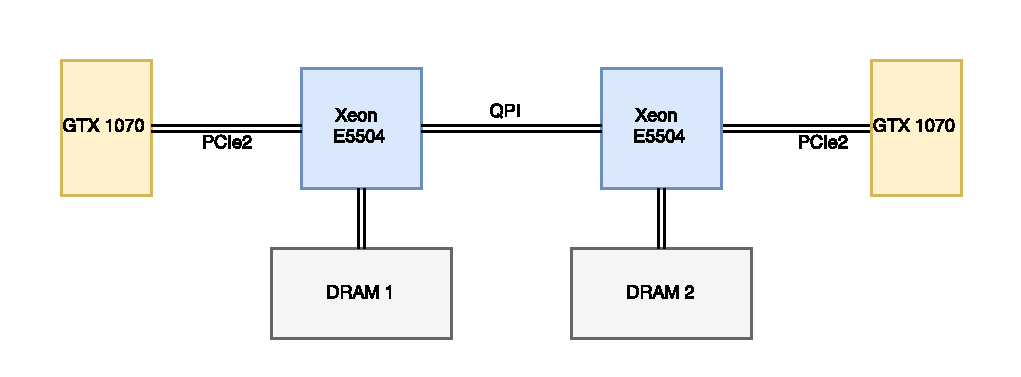
\includegraphics[width=.75\textwidth]{system}
	\label{f:sys}
	\caption{Test system, as described in chapter \ref{c:eval}. The QPI-Link between the two CPUs is the NUMA domain border.}
	\end{center}
\end{figure}
For Non-Uniform Memory Access(NUMA) architectures, research has shown that handling physical data locality has a positive influence on performance, yet few libraries and framework offer tools for fine-grained 
management of data locality. 
While in NVidia's CUDA framework device memory can be managed on a rather fine scale, host memory is treated as a single location, ignoring the possibility of underlying NUMA architectures.

In a system with multiple  NUMA-nodes, GPUs are either evenly distributed between all nodes or clustered on one or a few nodes. This connection to a node is the result of the PCIe controller that is part
	of the CPUs package. Regardless on how the system is configured, there are certain NUMA nodes, thus certain physical memory regions that are closer to one GPU than to a GPU that is connected to a different PCIe controller. Placing data on a NUMA node not directly connected to the GPU device causes lower host/device bandwidth due to indirection via HT/QPI for each memory access. An example for such a system is displayed in Figure \ref{f:sys}.

This project presents a way to explicitly set the NUMA-affinity for data allocations and movements with CUDA's unified memory. Chapter \ref{c:target} defines the goals of the project, and the means to reach them. Chapter \ref{c:env} presents the memory technologies and how they can be used and manipulated. Chapter \ref{c:impl} shows how these technologies are combined to achieve the defined goal. The resulting wrapper and the performance are evaluated in chapter \ref{c:eval}.

